\pdfoutput=1

\documentclass[11pt]{article}

\usepackage{EACL2023}

\usepackage{times}
\usepackage{latexsym}
\usepackage[T1]{fontenc}
\usepackage[utf8]{inputenc}
\usepackage{microtype}
\usepackage{graphicx}
\usepackage{booktabs}
\usepackage{amsmath}
\usepackage{multirow}
\usepackage{url}
\usepackage{xcolor}
\usepackage{enumitem}
\usepackage{array}

\newcommand{\todo}[1]{\textcolor{red}{[TODO: #1]}}

\title{Legal Clause Classification using Classical Models, Fine-Tuned Transformers, and Instruction-Tuned LLMs}

\author{
Yehoshua Benjamin Perez Condori \\
Student ID: 250057607 \\
MSc Artificial Intelligence \\
City St George's, University of London \\
\texttt{Yehoshua-Perez.Condori@city.ac.uk}
}

\begin{document}
\maketitle

\begin{abstract}
Legal contracts contain dense and technical language, making it difficult for non-experts to identify and interpret important contractual provisions. This coursework investigates Natural Language Processing methods for legal clause classification using LEDGAR, a pre-annotated dataset of contract provisions. The task is framed as supervised clause type classification rather than legal risk prediction, unfairness detection, or enforceability assessment, since those tasks would require specialist legal judgement and dedicated legal-risk labels.

The project compares three levels of NLP methods: classical TF-IDF-based models, a fine-tuned transformer model, and instruction-tuned large language model prompting using Qwen2.5-Instruct. Models are evaluated using accuracy, macro-F1, weighted-F1, per-class performance, confusion matrices, and invalid prediction rate for the prompted LLM. The results show that \todo{insert main result after experiments}. Error analysis examines class imbalance, overlapping legal terminology, ambiguous clause wording, and failure cases in both supervised and prompted classification.
\end{abstract}

\section{Introduction}

Legal contracts are central to commercial and professional relationships, but their dense and technical language can make them difficult to review efficiently. Important clauses may define governing law, confidentiality obligations, indemnification duties, termination rights, assignment rules, notice requirements, limitation of liability, and other legally significant provisions. These clauses are often embedded within long documents and may use repeated boilerplate wording, subtle legal distinctions, or domain-specific terminology.

This coursework investigates how Natural Language Processing (NLP) can be used to classify legal contract clauses into predefined clause categories. The project does not attempt to predict legal risk, unfairness, or enforceability. Such tasks would require expert legal judgement and dedicated legal risk labels. Instead, this project focuses on clause type classification, which is a clearer and more measurable supervised learning task.

The project compares three levels of NLP methods. First, classical supervised machine learning models are trained using TF-IDF features. Second, a transformer model is fine-tuned for sequence classification. Third, an instruction-tuned large language model, Qwen2.5-Instruct, is evaluated as a prompting baseline. This comparison allows the coursework to examine whether traditional sparse text-classification methods remain competitive against more recent transformer-based and instruction-following models for controlled legal clause classification.

The main contributions of this coursework are:

\begin{itemize}[leftmargin=*]
    \item a reproducible pipeline for legal clause classification using LEDGAR;
    \item a comparison of dummy baselines, classical models, a fine-tuned transformer model, and instruction-tuned LLM prompting;
    \item an evaluation of whether supervised training outperforms prompting for controlled multiclass legal classification;
    \item an analysis of class imbalance, label ambiguity, invalid LLM outputs, and model failure cases;
    \item a discussion of how confidence-based review could support human-in-the-loop contract triage.
\end{itemize}

\section{Research Questions}

This coursework addresses the following research questions:

\begin{enumerate}[leftmargin=*]
    \item How well do classical machine-learning models perform on legal clause classification compared with a fine-tuned transformer model?
    
    \item Can an instruction-tuned LLM such as Qwen2.5-Instruct classify legal clauses effectively using zero-shot or few-shot prompting without task-specific fine-tuning?
    
    \item What clause categories are most difficult to classify, and are errors mainly caused by class imbalance, overlapping legal terminology, or label ambiguity?

    \item How can confidence scores and invalid-output analysis be used to identify predictions that may require human review?
\end{enumerate}

The hypothesis is that TF-IDF with Linear SVM will provide a strong classical baseline because legal clauses often contain repeated wording and distinctive phrase patterns. Fine-tuned transformer models are expected to perform better on semantically subtle categories where context matters more than keywords. Qwen2.5-Instruct is expected to perform reasonably in few-shot settings, especially for common and clearly named labels. However, it may produce invalid labels, overly general categories, or semantically plausible but non-matching predictions.

\section{Background and Related Work}

Legal NLP is challenging because legal text contains formal vocabulary, long sentences, repeated boilerplate language, and subtle distinctions between similar legal provisions. Clause classification is useful because it can organise contract content and support faster human review.

The Contract Understanding Atticus Dataset (CUAD) is an important legal NLP dataset containing expert annotations for contract review \citep{hendrycks2021cuad}. However, CUAD is primarily structured around contract review and span extraction rather than direct multiclass classification. For this reason, CUAD was considered as a possible secondary dataset but was not used as the main dataset in the experimental pipeline.

LEDGAR is more directly suitable for this coursework because it contains legal provisions labelled by clause type \citep{tuggener2020ledgar}. Each instance can be treated as a text classification example, making it appropriate for comparing supervised NLP models.

Classical machine learning approaches remain strong baselines for text classification, especially when categories contain distinctive lexical patterns. Prior work on clause topic classification has shown that BERT-based models can achieve strong performance, but logistic regression can also remain competitive \citep{braun2022clause}. Transformer models such as BERT \citep{devlin2019bert}, DistilBERT \citep{sanh2019distilbert}, and LegalBERT \citep{chalkidis2020legalbert} provide contextual representations that may capture legal meaning better than sparse bag-of-words features.

Recent instruction-tuned large language models also make it possible to test classification through prompting rather than fine-tuning. Qwen2.5 is a family of large language models released in base and instruction-tuned variants \citep{yang2025qwen25}. This project evaluates Qwen2.5-Instruct as a prompting baseline for legal clause classification.

\section{Dataset}

\subsection{Primary Dataset: LEDGAR}

The primary dataset is LEDGAR, a legal clause classification dataset containing contract provisions labelled by clause type. Each example consists of clause text and a corresponding label. The task is therefore formulated as multiclass text classification.

The dataset was loaded from the Hugging Face Hub dataset \texttt{coastalchp/ledgar} using the Hugging Face \texttt{datasets} library. This version is provided in Hugging Face/Parquet format and contains predefined train, validation, and test splits. The raw dataset contains 80,000 examples across 100 clause labels, with 60,000 training examples, 10,000 validation examples, and 10,000 test examples.

\subsection{Label Selection}

To keep the experiment computationally manageable and reduce extreme class imbalance, this coursework focuses on the top 20 most frequent clause categories. These categories are selected using the training split only. This prevents information from the validation or test sets from influencing the final label space.

After filtering, the processed dataset contains only examples whose labels belong to the top 20 most frequent clause categories in the training split. The final filtered counts are generated by the preprocessing notebook and reported in Table~\ref{tab:dataset-stats}.

Each processed example follows the schema:

\begin{itemize}[leftmargin=*]
    \item \texttt{text}
    \item \texttt{label}
    \item \texttt{label\_id}
    \item \texttt{split}
    \item \texttt{source\_dataset}
\end{itemize}

\begin{table}[t]
\centering
\small
\begin{tabular}{lr}
\toprule
\textbf{Dataset Statistic} & \textbf{Value} \\
\midrule
Raw examples & 80,000 \\
Raw labels & 100 \\
Original train examples & 60,000 \\
Original validation examples & 10,000 \\
Original test examples & 10,000 \\
Final examples & \todo{value from preprocessing output} \\
Final labels & 20 \\
Filtered train examples & \todo{value} \\
Filtered validation examples & \todo{value} \\
Filtered test examples & \todo{value} \\
Average clause length & \todo{value} \\
Maximum clause length & \todo{value} \\
\bottomrule
\end{tabular}
\caption{Summary statistics for the LEDGAR dataset and the processed top-20-label classification subset.}
\label{tab:dataset-stats}
\end{table}

\begin{figure}[t]
\centering
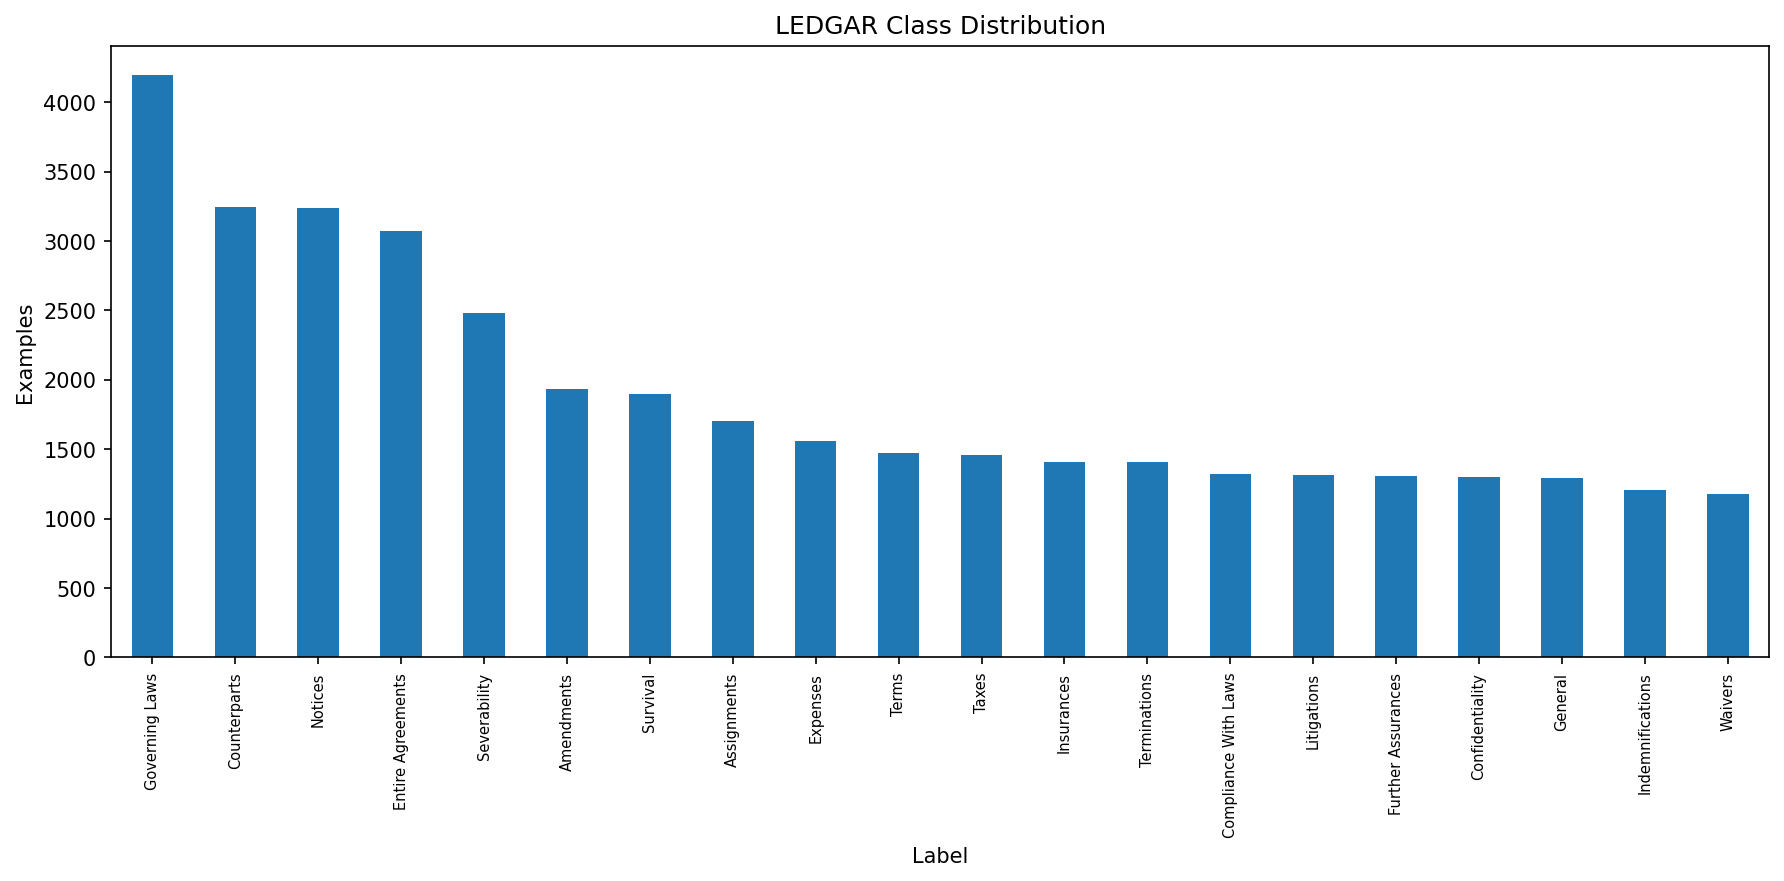
\includegraphics[width=\linewidth]{figures/label_distribution.png}
\caption{Distribution of the top 20 LEDGAR clause categories after filtering. This figure shows the class imbalance present in the final classification dataset.}
\label{fig:label-distribution}
\end{figure}

\begin{figure}[t]
\centering
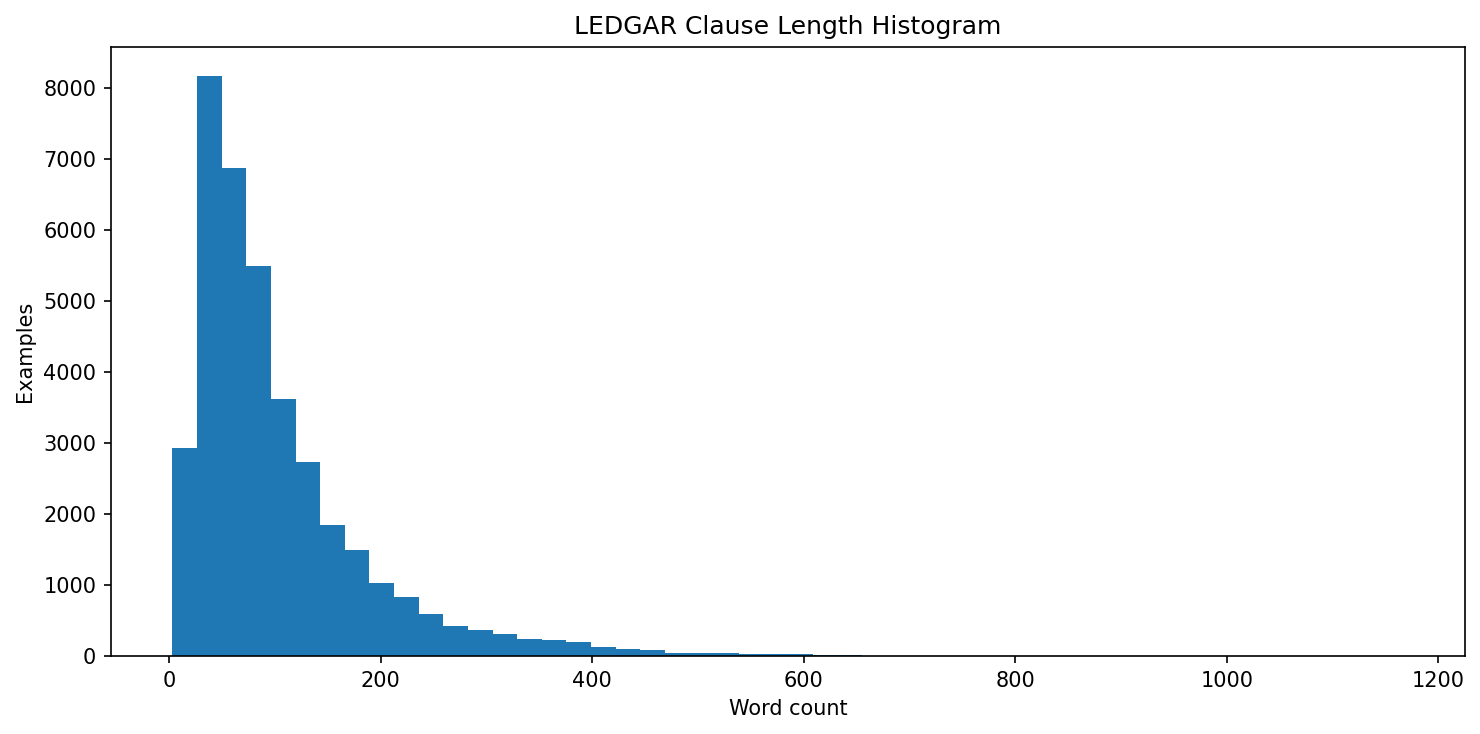
\includegraphics[width=\linewidth]{figures/clause_length_distribution.png}
\caption{Distribution of clause lengths in the processed LEDGAR dataset. This figure is used to justify the selected transformer maximum sequence length.}
\label{fig:clause-length}
\end{figure}

\subsection{Considered Secondary Dataset: CUAD}

CUAD was considered as a possible secondary dataset because it contains expert annotations for contract review. However, it was not treated as the main classification dataset because it was originally designed for contract review and span extraction rather than direct multiclass clause classification.

The main experimental pipeline therefore uses LEDGAR only. CUAD remains relevant as related work and as a possible future extension for external validation or span-to-label adaptation.

\section{Preprocessing}

The preprocessing pipeline includes:

\begin{itemize}[leftmargin=*]
    \item loading LEDGAR from \texttt{coastalchp/ledgar} on the Hugging Face Hub;
    \item preserving the predefined train, validation, and test splits;
    \item standardising column names;
    \item normalising whitespace while preserving legal punctuation;
    \item removing empty or malformed examples;
    \item removing duplicate text-label pairs;
    \item analysing label distributions;
    \item selecting the top 20 labels from the training split only;
    \item encoding labels into numerical IDs;
    \item saving processed train, validation, and test files;
    \item generating dataset summary outputs and figures.
\end{itemize}

For classical models, clause text is converted into TF-IDF vectors using unigram and bigram features. For transformer models, clause text is tokenised using the relevant Hugging Face tokenizer with padding and truncation. A maximum sequence length of 256 tokens is used to keep transformer training computationally manageable while still covering most clause texts.

For Qwen2.5-Instruct prompting, no manual feature extraction is performed. Instead, the prompt includes the task instruction, allowed label list, and clause text.

\section{Models}

\subsection{Dummy Baselines}

Two non-trained baselines are used.

\paragraph{Majority Class Baseline.}
This baseline always predicts the most frequent training label. It exposes the effect of class imbalance and provides a minimum expected comparison point.

\paragraph{Random Baseline.}
This baseline predicts labels randomly using the training label distribution, so more frequent clause categories are sampled more often. It checks whether trained models perform meaningfully better than chance.

\subsection{Classical Machine Learning Models}

The classical models are trained using TF-IDF features:

\begin{itemize}[leftmargin=*]
    \item TF-IDF + Logistic Regression;
    \item TF-IDF + Linear SVM;
    \item TF-IDF + Multinomial Naive Bayes;
    \item optionally, TF-IDF + Complement Naive Bayes.
\end{itemize}

These models are included because they are efficient, interpretable, and strong baselines for text classification. Hyperparameter tuning considers:

\begin{itemize}[leftmargin=*]
    \item maximum TF-IDF features;
    \item unigram versus unigram-bigram features;
    \item regularisation strength \(C\);
    \item class weighting;
    \item Naive Bayes smoothing parameter \(\alpha\).
\end{itemize}

Model selection is based on validation macro-F1.

\subsection{Fine-Tuned Transformer Model}

One transformer model is fine-tuned for sequence classification. The candidate models considered were:

\begin{itemize}[leftmargin=*]
    \item \texttt{distilbert-base-uncased};
    \item \texttt{nlpaueb/legal-bert-base-uncased};
    \item \texttt{nlpaueb/bert-base-uncased-contracts}.
\end{itemize}

DistilBERT is the safest option if GPU resources are limited. LegalBERT or a contract-specific BERT model is more domain-aligned if computational resources allow. The final transformer used in the experiment was \todo{insert final transformer model used}.

The transformer experiment uses:

\begin{itemize}[leftmargin=*]
    \item Hugging Face tokenizer;
    \item \texttt{AutoModelForSequenceClassification};
    \item PyTorch backend;
    \item validation-based model selection;
    \item macro-F1 as the main metric.
\end{itemize}

The transformer hyperparameters are shown in Table~\ref{tab:hyperparameters}.

\subsection{Qwen2.5-Instruct Prompting Baseline}

Qwen2.5-Instruct is used as a prompting baseline and is not fine-tuned. The purpose of this experiment is to test whether an instruction-tuned LLM can perform legal clause classification without task-specific supervised training.

The prompt provides:

\begin{itemize}[leftmargin=*]
    \item a task instruction;
    \item the full list of allowed labels;
    \item the clause text;
    \item an instruction to return exactly one label.
\end{itemize}

Zero-shot prompting uses no examples. Few-shot prompting uses training examples only, ideally one example per class where possible. Due to computational cost, the Qwen experiment is evaluated on a smaller test sample when full-test inference is not feasible.

A simplified prompt template is shown below:

\begin{quote}
You are classifying legal contract clauses. Choose exactly one label from the allowed label list. Do not invent new labels.

Allowed labels: \todo{insert top-20 label list}

Clause: \todo{insert example clause text}

Answer with exactly one label:
\end{quote}

\section{Confidence-Based Review Demonstration}

A small confidence-based review workflow is discussed as a practical extension to the classification system. The workflow is designed for clause triage rather than autonomous legal decision-making:

\begin{center}
\begin{tabular}{c}
Input clause \\
$\downarrow$ \\
Best classifier predicts clause type \\
$\downarrow$ \\
Confidence score or margin is calculated \\
$\downarrow$ \\
Low-confidence prediction is flagged \\
$\downarrow$ \\
Output: predicted label, confidence, and review flag \\
\end{tabular}
\end{center}

This is framed as a research prototype for human-in-the-loop contract review. It does not provide legal advice and should not be interpreted as a production-ready legal tool.

If implemented, predictions are flagged for review when confidence falls below a predefined threshold. For linear models, confidence may be estimated using probability scores or decision margins. For the transformer model, softmax confidence can be used.

\begin{figure}[t]
\centering
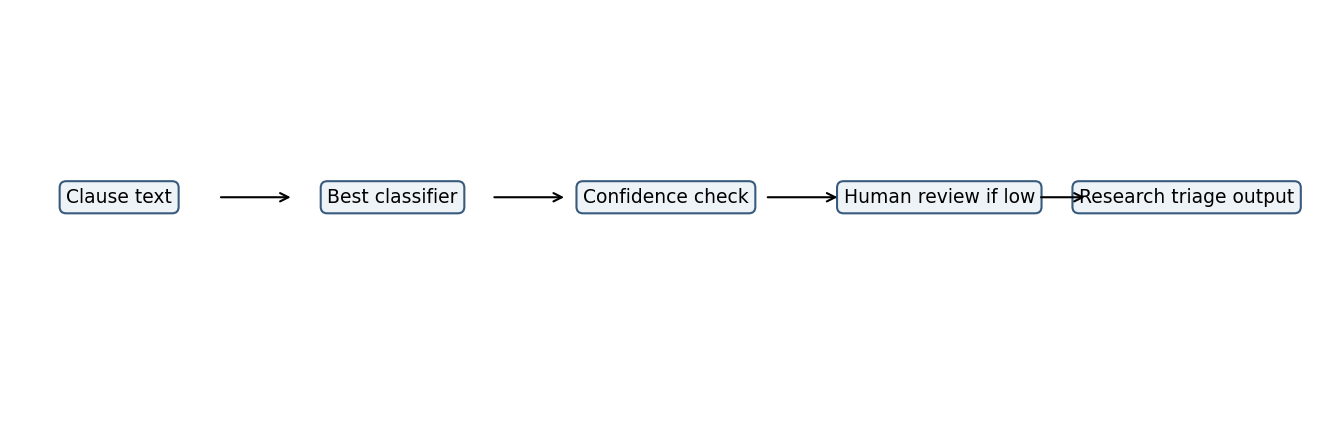
\includegraphics[width=\linewidth]{figures/agentic_review_workflow.png}
\caption{Confidence-based review workflow. Low-confidence predictions are flagged for human review rather than treated as final legal decisions.}
\label{fig:agentic-workflow}
\end{figure}

\section{Experimental Setup}

All experiments are implemented in Python. The main tools are:

\begin{itemize}[leftmargin=*]
    \item Pandas and NumPy for data handling;
    \item Scikit-learn for TF-IDF, classical models, metrics, and confusion matrices;
    \item Hugging Face Datasets for dataset loading;
    \item Hugging Face Transformers for transformer training and Qwen inference;
    \item PyTorch for transformer training and inference;
    \item Matplotlib for visualisation;
    \item Optuna optionally for hyperparameter optimisation.
\end{itemize}

Experiments are implemented in a Python notebook environment. Classical models are run using CPU-based Scikit-learn, while transformer fine-tuning and Qwen2.5-Instruct inference use GPU acceleration when CUDA is available. The notebook records the detected hardware configuration for reproducibility. Random seeds are fixed where possible to improve reproducibility.

\begin{table}[t]
\centering
\small
\begin{tabular}{ll}
\toprule
\textbf{Component} & \textbf{Tool} \\
\midrule
Data handling & Pandas, NumPy \\
Classical models & Scikit-learn \\
Transformer training & Hugging Face Transformers, PyTorch \\
LLM prompting & Qwen2.5-Instruct \\
Evaluation & Scikit-learn metrics \\
Visualisation & Matplotlib \\
Hyperparameter tuning & Grid search / Optuna \\
Environment & Python notebook with optional CUDA GPU acceleration \\
\bottomrule
\end{tabular}
\caption{Tools used in the experimental pipeline.}
\label{tab:tools}
\end{table}

\section{Evaluation Metrics}

The main evaluation metrics are:

\begin{itemize}[leftmargin=*]
    \item accuracy;
    \item macro-F1;
    \item weighted-F1;
    \item per-class precision, recall, and F1-score;
    \item confusion matrix;
    \item invalid prediction rate for Qwen2.5-Instruct.
\end{itemize}

Macro-F1 is treated as the primary metric because the dataset is imbalanced. Weighted-F1 is also reported to show performance while accounting for label frequency.

For the Qwen experiment, invalid predictions are analysed separately. An invalid prediction occurs when the model returns a label outside the allowed label set, produces multiple labels, or gives an explanation instead of the required single label.

\section{Results}

Table~\ref{tab:main-results} reports the main test-set results.

\begin{table}[t]
\centering
\small
\begin{tabular}{lcccc}
\toprule
\textbf{Model} & \textbf{Accuracy} & \textbf{Macro-F1} & \textbf{Weighted-F1} & \textbf{Invalid Rate} \\
\midrule
Majority baseline & \todo{value} & \todo{value} & \todo{value} & -- \\
Random baseline & \todo{value} & \todo{value} & \todo{value} & -- \\
TF-IDF + Naive Bayes & \todo{value} & \todo{value} & \todo{value} & -- \\
TF-IDF + Logistic Regression & \todo{value} & \todo{value} & \todo{value} & -- \\
TF-IDF + Linear SVM & \todo{value} & \todo{value} & \todo{value} & -- \\
\todo{DistilBERT / LegalBERT} & \todo{value} & \todo{value} & \todo{value} & -- \\
Qwen2.5 zero-shot & \todo{value} & \todo{value} & \todo{value} & \todo{value} \\
Qwen2.5 few-shot & \todo{value} & \todo{value} & \todo{value} & \todo{value} \\
\bottomrule
\end{tabular}
\caption{Test-set performance of baselines, classical models, fine-tuned transformer model, and Qwen2.5 prompting baselines. Macro-F1 is the primary metric.}
\label{tab:main-results}
\end{table}

\begin{figure}[t]
\centering
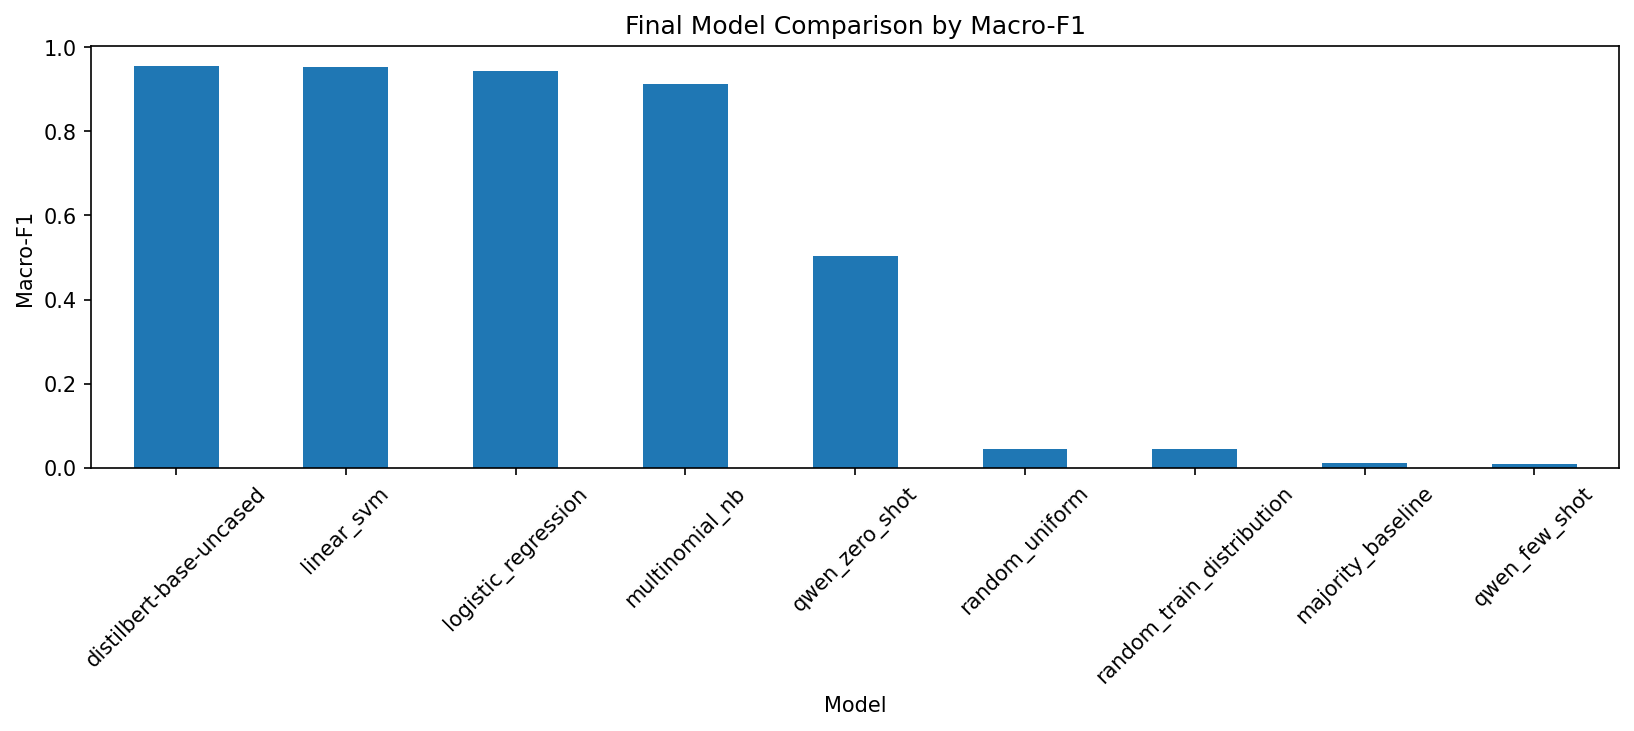
\includegraphics[width=\linewidth]{figures/model_comparison_macro_f1.png}
\caption{Macro-F1 comparison across dummy baselines, classical models, the fine-tuned transformer model, and Qwen2.5 prompting baselines.}
\label{fig:model-comparison}
\end{figure}

The results show that \todo{insert best model and key score from main_results.csv}. The majority and random baselines perform \todo{insert interpretation}, showing whether the task can be solved by exploiting label frequency alone.

Among the classical models, \todo{insert strongest classical model} performs best. This suggests that \todo{explain using observed results}. The transformer model \todo{outperforms / does not outperform} the strongest classical model, suggesting that \todo{interpret whether contextual modelling helped based on results}.

The Qwen2.5-Instruct prompting baseline achieves \todo{insert result}. Few-shot prompting \todo{improves / does not improve} performance compared with zero-shot prompting. Invalid prediction rate is important because prompted LLMs may produce labels outside the controlled label set.

\begin{figure}[t]
\centering
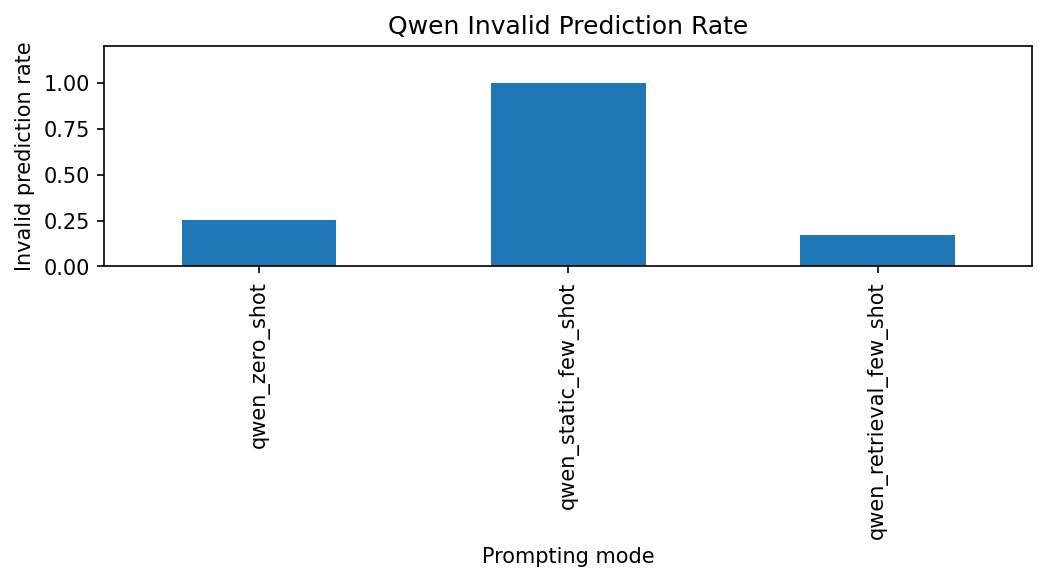
\includegraphics[width=\linewidth]{figures/qwen_invalid_predictions.png}
\caption{Invalid prediction rate for Qwen2.5-Instruct under zero-shot and few-shot prompting. Invalid outputs include labels outside the allowed label set, multiple labels, or explanatory text instead of a single label.}
\label{fig:qwen-invalid}
\end{figure}

\section{Per-Class Analysis}

Table~\ref{tab:per-class} shows per-class scores for selected clause categories using the best-performing model.

\begin{table}[t]
\centering
\small
\begin{tabular}{lccc}
\toprule
\textbf{Clause Category} & \textbf{Precision} & \textbf{Recall} & \textbf{F1} \\
\midrule
\todo{Class 1} & \todo{value} & \todo{value} & \todo{value} \\
\todo{Class 2} & \todo{value} & \todo{value} & \todo{value} \\
\todo{Class 3} & \todo{value} & \todo{value} & \todo{value} \\
\todo{Class 4} & \todo{value} & \todo{value} & \todo{value} \\
\todo{Class 5} & \todo{value} & \todo{value} & \todo{value} \\
\bottomrule
\end{tabular}
\caption{Per-class performance for selected clause categories using the best-performing model.}
\label{tab:per-class}
\end{table}

The strongest categories are \todo{insert categories from per-class results}. These categories may contain distinctive legal phrases or repeated boilerplate wording. The weakest categories are \todo{insert categories from per-class results}. These may be harder because of class imbalance, semantic overlap, or ambiguous clause wording.

\section{Error Analysis}

Error analysis is conducted using confusion matrices, misclassified examples, and invalid Qwen outputs.

\subsection{Confusion Matrix}

Figure~\ref{fig:confusion-matrix-best} shows the confusion matrix for the best-performing supervised model.

\begin{figure}[t]
\centering
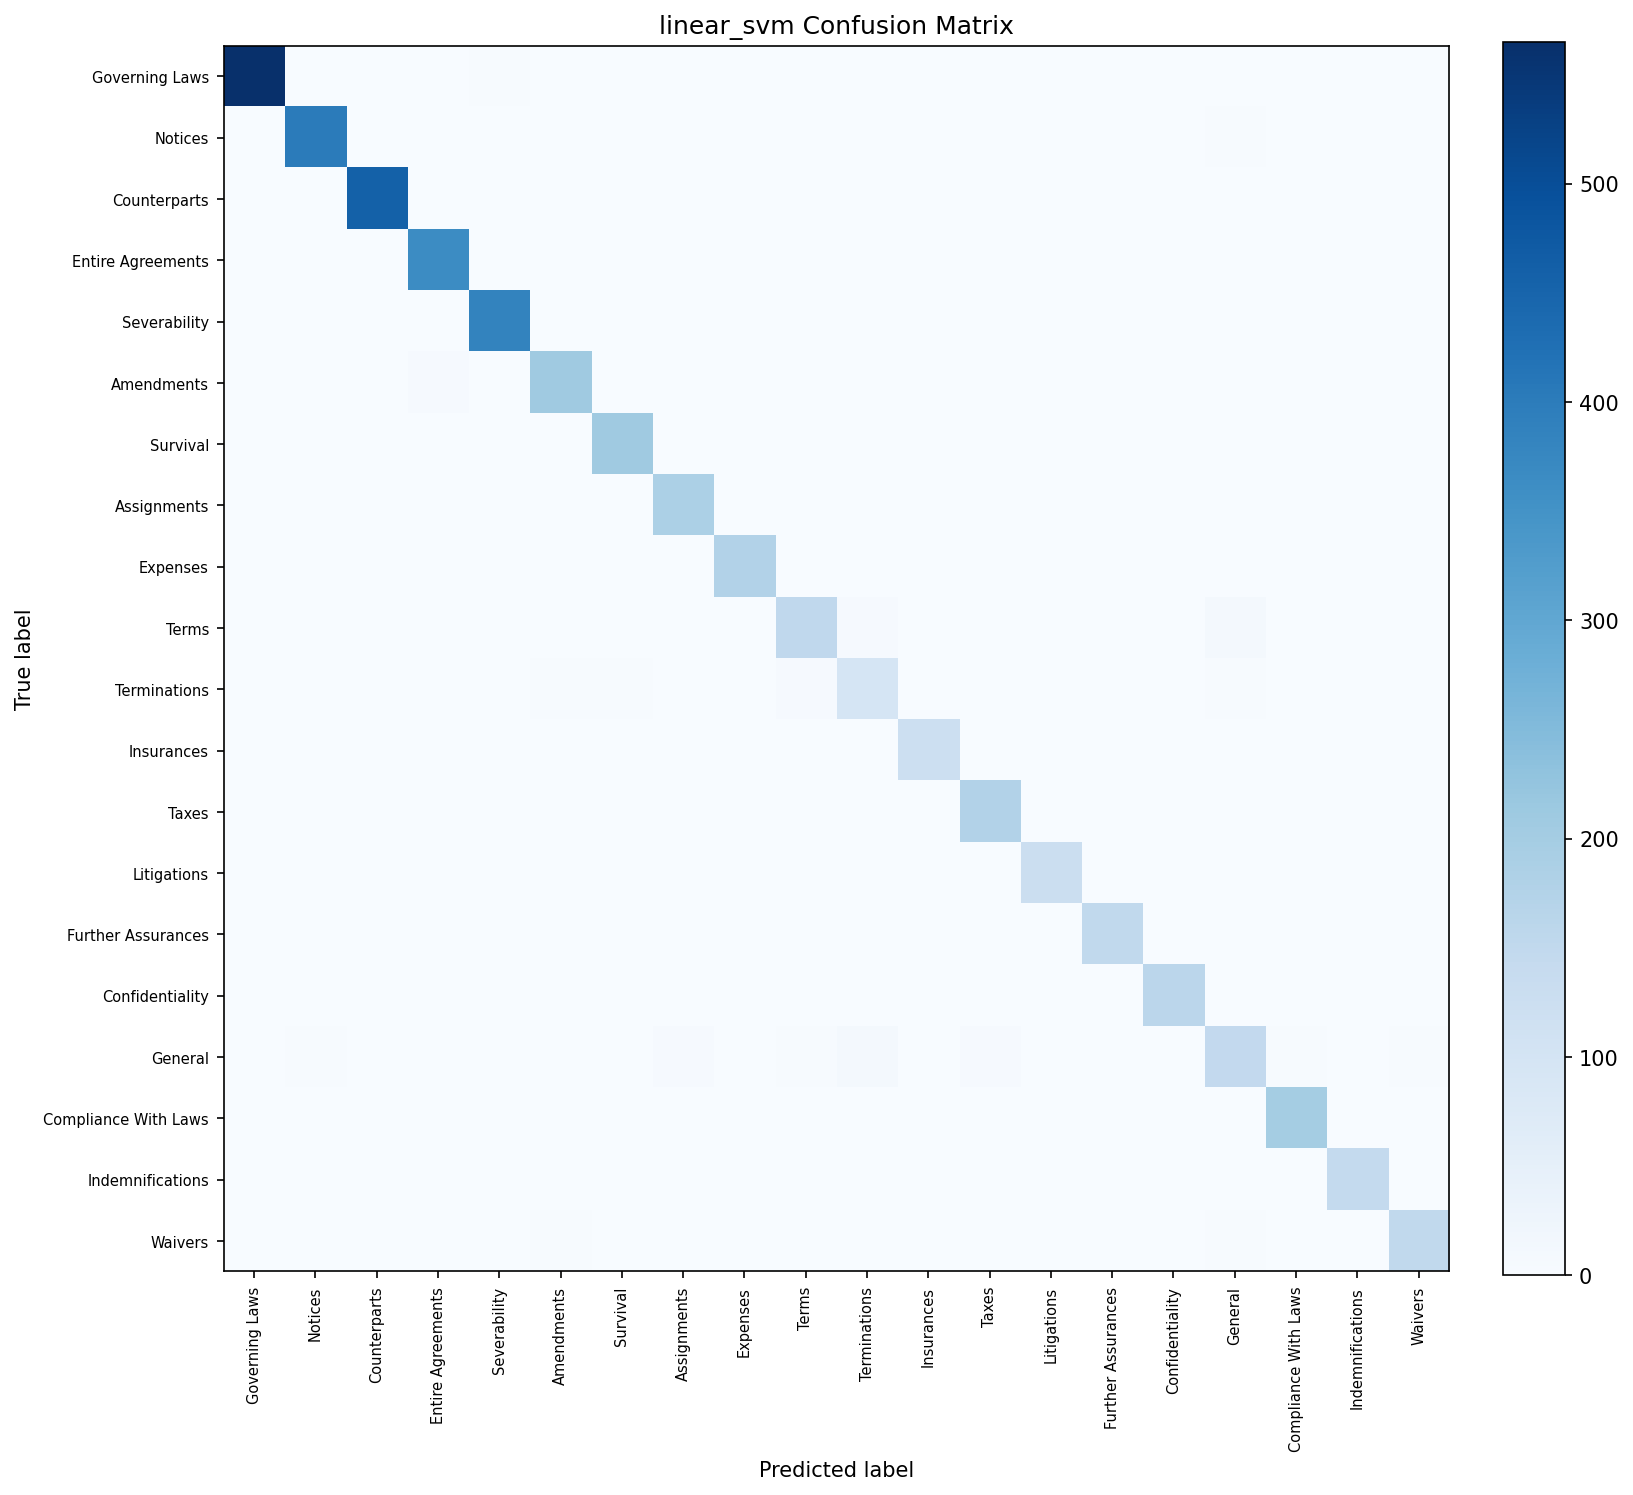
\includegraphics[width=\linewidth]{figures/confusion_matrix_best_model.png}
\caption{Confusion matrix for the best-performing supervised model on the test set. The matrix highlights which clause categories are most frequently confused.}
\label{fig:confusion-matrix-best}
\end{figure}

The most commonly confused label pairs are:

\begin{itemize}[leftmargin=*]
    \item \todo{Label A} and \todo{Label B};
    \item \todo{Label C} and \todo{Label D};
    \item \todo{Label E} and \todo{Label F}.
\end{itemize}

These confusions suggest that some clause categories share overlapping legal vocabulary or similar functional meaning.

\subsection{Classical Model Errors}

The best classical model makes errors when clauses contain generic legal terms shared across several categories. TF-IDF models rely heavily on surface-level word patterns, so they may struggle when the same terms appear in different clause types.

\subsection{Transformer Model Errors}

The transformer model can handle context better than classical models, but it may still fail on long clauses, ambiguous wording, or categories with fewer training examples. If clauses are truncated, useful information near the end of a clause may be lost.

\subsection{Qwen2.5-Instruct Errors}

The Qwen2.5-Instruct baseline is analysed separately because prompted LLMs can fail in different ways. Errors include:

\begin{itemize}[leftmargin=*]
    \item returning a label outside the allowed label set;
    \item returning multiple labels instead of one;
    \item giving an explanation instead of a label;
    \item predicting a semantically plausible but non-matching label;
    \item overgeneralising from clause wording.
\end{itemize}

\begin{table}[t]
\centering
\small
\begin{tabular}{p{0.34\linewidth}lll}
\toprule
\textbf{Clause Text} & \textbf{Gold Label} & \textbf{Prediction} & \textbf{Error Type} \\
\midrule
\todo{shortened clause} & \todo{label} & \todo{label} & \todo{reason} \\
\todo{shortened clause} & \todo{label} & \todo{label} & \todo{reason} \\
\todo{shortened clause} & \todo{label} & \todo{label} & \todo{reason} \\
\bottomrule
\end{tabular}
\caption{Example misclassifications from the best-performing model or Qwen baseline.}
\label{tab:misclassifications}
\end{table}

\section{Confidence-Based Review Demonstration}

The confidence-based review workflow is evaluated as a prototype rather than a core classifier if implementation outputs are available. The goal is to show how a model could support human-in-the-loop contract triage.

The system flags predictions for review when confidence is below \todo{threshold, if implemented}. For linear models, confidence may be estimated using probability scores or decision margins. For the transformer model, softmax confidence is used. Any LLM-generated supporting phrase is treated only as an explanatory aid and is not legally authoritative.

\begin{table}[t]
\centering
\small
\begin{tabular}{llll}
\toprule
\textbf{Clause} & \textbf{Prediction} & \textbf{Confidence} & \textbf{Review Flag} \\
\midrule
\todo{short clause} & \todo{label} & \todo{0.xx} & Yes \\
\todo{short clause} & \todo{label} & \todo{0.xx} & No \\
\todo{short clause} & \todo{label} & \todo{0.xx} & Yes \\
\bottomrule
\end{tabular}
\caption{Example outputs from the confidence-based review prototype.}
\label{tab:agentic-review}
\end{table}

This extension demonstrates practical triage but should not be interpreted as a production-ready legal tool.

\section{Discussion}

The results show that \todo{summarise main finding using actual result values}. If Linear SVM performs strongly, this supports the hypothesis that legal clause categories often contain distinctive wording that can be captured by TF-IDF features. If the transformer model improves macro-F1, this suggests that contextual representations help with semantically subtle clause categories. If the transformer model does not improve substantially, this may indicate that the top-20 LEDGAR categories are strongly lexical and can be handled effectively by sparse classical features.

The Qwen2.5-Instruct experiment provides a useful comparison between supervised classification and prompting. If Qwen performs well in few-shot settings, this suggests that instruction-tuned LLMs can classify some legal clauses without task-specific fine-tuning. However, invalid prediction rate and strict label matching remain important limitations. In controlled multiclass evaluation, supervised models have the advantage of always predicting from the allowed label set.

The confidence-based review workflow shows how classification could support human review. However, the system does not provide legal advice and should only be viewed as a research prototype.

\section{Limitations}

This project has several limitations.

First, it does not predict legal risk, unfairness, or enforceability. It only classifies clause types. Any discussion of legal importance is used as motivation rather than as a supervised prediction target.

Second, the dataset is imbalanced. Some clause categories have many more examples than others, which can affect performance and make rare categories difficult to evaluate.

Third, only one fine-tuned transformer model is used due to time and computational constraints. A broader comparison could evaluate more transformer architectures.

Fourth, Qwen2.5-Instruct may be evaluated on a smaller test sample because LLM inference is more computationally expensive than classical model prediction.

Fifth, the confidence-based review workflow is only a demonstration. It is not a legal advisor and should not be used for real contract decision-making.

\section{Conclusion}

This coursework investigated legal clause classification using classical models, a fine-tuned transformer model, and instruction-tuned LLM prompting. LEDGAR was used as the main supervised dataset, while CUAD was considered as a possible secondary dataset but was not used in the main experimental pipeline.

The best-performing model was \todo{insert model name}, achieving a macro-F1 score of \todo{value}. The findings show that \todo{insert final conclusion}. Classical TF-IDF models provide efficient and competitive baselines, while fine-tuned transformers may offer advantages for semantically complex clauses. Qwen2.5-Instruct provides a flexible prompting baseline, but invalid labels and strict label matching remain important challenges.

Overall, the project demonstrates that NLP can support legal contract review by automatically categorising clause types. However, automated clause classification should be treated as a decision-support tool rather than a replacement for human legal judgement.

\section*{Reproducibility Statement}

The coursework code includes dataset loading, preprocessing, model training, evaluation, prediction saving, and visualisation. Random seeds were fixed where possible. The final results can be reproduced by running the main experimental notebook, which loads LEDGAR from Hugging Face, applies the top-20-label filtering pipeline, trains the baseline and supervised models, evaluates predictions, and saves the result tables and figures used in this report.

\bibliographystyle{acl_natbib}
\begin{thebibliography}{}

\bibitem[Braun and Matthes(2022)]{braun2022clause}
Daniel Braun and Florian Matthes. 2022.
\newblock Clause topic classification in German and English standard form contracts.
\newblock In \textit{Proceedings of the Fifth Workshop on e-Commerce and NLP}, pages 199--209.

\bibitem[Chalkidis et~al.(2020)]{chalkidis2020legalbert}
Ilias Chalkidis, Manos Fergadiotis, Prodromos Malakasiotis, Nikolaos Aletras, and Ion Androutsopoulos. 2020.
\newblock LEGAL-BERT: The muppets straight out of law school.
\newblock In \textit{Findings of EMNLP}.

\bibitem[Chalkidis et~al.(2022)]{chalkidis2022lexglue}
Ilias Chalkidis, Abhik Jana, Dirk Hartung, Michael Bommarito, Ion Androutsopoulos, Daniel Katz, and Nikolaos Aletras. 2022.
\newblock LexGLUE: A benchmark dataset for legal language understanding in English.
\newblock In \textit{Proceedings of ACL}.

\bibitem[Devlin et~al.(2019)]{devlin2019bert}
Jacob Devlin, Ming-Wei Chang, Kenton Lee, and Kristina Toutanova. 2019.
\newblock BERT: Pre-training of deep bidirectional transformers for language understanding.
\newblock In \textit{Proceedings of NAACL-HLT}, pages 4171--4186.

\bibitem[Hendrycks et~al.(2021)]{hendrycks2021cuad}
Dan Hendrycks, Collin Burns, Anya Chen, and Spencer Ball. 2021.
\newblock CUAD: An expert-annotated NLP dataset for legal contract review.
\newblock In \textit{Proceedings of NeurIPS Datasets and Benchmarks Track}.

\bibitem[Sanh et~al.(2019)]{sanh2019distilbert}
Victor Sanh, Lysandre Debut, Julien Chaumond, and Thomas Wolf. 2019.
\newblock DistilBERT, a distilled version of BERT: smaller, faster, cheaper and lighter.
\newblock \textit{arXiv preprint arXiv:1910.01108}.

\bibitem[Tuggener et~al.(2020)]{tuggener2020ledgar}
Don Tuggener, Pius von D{\"a}niken, Thomas Peetz, and Mark Cieliebak. 2020.
\newblock LEDGAR: A large-scale multi-label corpus for text classification of legal provisions in contracts.
\newblock In \textit{Proceedings of the 12th Language Resources and Evaluation Conference}.

\bibitem[Yang et~al.(2025)]{yang2025qwen25}
An Yang, Baosong Yang, Beichen Zhang, Binyuan Hui, Bo Zheng, Bowen Yu, Chengyuan Li, Dayiheng Liu, Fei Huang, Haoran Wei, Huan Lin, Jian Yang, Jianhong Tu, Jianwei Zhang, Jianxin Yang, Jiaxi Yang, Jingren Zhou, Junyang Lin, Kai Dang, Keming Lu, Keqin Bao, Kexin Yang, Le Yu, Mei Li, Mingfeng Xue, Pei Zhang, Qin Zhu, Rui Men, Runji Lin, Tianhao Li, Tianyi Tang, Tingyu Xia, Xingzhang Ren, Xuancheng Ren, Yang Fan, Yang Su, Yichang Zhang, Yu Wan, Yuqiong Liu, Zeyu Cui, Zhenru Zhang, Zihan Qiu, and others. 2025.
\newblock Qwen2.5 Technical Report.
\newblock \textit{arXiv preprint arXiv:2412.15115}.

\end{thebibliography}

\appendix

\section{Appendix A: Hyperparameters}

\begin{table}[h]
\centering
\small
\begin{tabular}{lll}
\toprule
\textbf{Model} & \textbf{Parameter} & \textbf{Value} \\
\midrule
TF-IDF & n-gram range & (1, 2) \\
TF-IDF & max features & 50,000 \\
Logistic Regression & C & 1.0 \\
Logistic Regression & class weight & balanced \\
Linear SVM & C & 1.0 \\
Linear SVM & class weight & balanced \\
Multinomial NB & alpha & 1.0 \\
Transformer & model name & \todo{value} \\
Transformer & learning rate & 2e-5 \\
Transformer & batch size & 16 \\
Transformer & epochs & 3 \\
Transformer & max sequence length & 256 \\
Qwen2.5 & model size & \todo{value} \\
Qwen2.5 & zero-shot sample size & \todo{value} \\
Qwen2.5 & few-shot sample size & \todo{value} \\
\bottomrule
\end{tabular}
\caption{Hyperparameters used in the experiments.}
\label{tab:hyperparameters}
\end{table}

\section{Appendix B: Qwen Prompt Template}

\begin{quote}
You are classifying legal contract clauses.

Choose exactly one label from the allowed label list.

Allowed labels:
\texttt{[top-20 LEDGAR labels generated from the training split]}

Clause:
\texttt{[clause text]}

Return exactly one label and nothing else.
\end{quote}

\section{Appendix C: Example Misclassifications}

\begin{table}[h]
\centering
\small
\begin{tabular}{p{0.36\linewidth}lll}
\toprule
\textbf{Clause Text} & \textbf{Gold Label} & \textbf{Prediction} & \textbf{Likely Cause} \\
\midrule
\todo{shortened clause} & \todo{label} & \todo{label} & \todo{reason} \\
\todo{shortened clause} & \todo{label} & \todo{label} & \todo{reason} \\
\todo{shortened clause} & \todo{label} & \todo{label} & \todo{reason} \\
\bottomrule
\end{tabular}
\caption{Examples of misclassified clauses.}
\label{tab:appendix-misclassifications}
\end{table}

\end{document}
